\section{Bayesian networks}
\subsection{The Bayes' theorem}
The theorem stated by Thomas Bayes says that, given two events $H$ (hypothesis) and $T$ (thesis), respectively with probabilities $P(H)$ and $P(T)$:
\[ P(H|T) = \frac{P(H \cap T)}{P(T)} = \frac{P(T|H)P(H)}{P(T)}, \]
that is: the probability that the hypothesis is verified, given that we know the thesis, comes from the probability of observing the thesis knowing the hypothesis occurred, times the ratio of the single probabilities of hypothesis over the thesis.

We call $P(H)$ the \textit{prior} probability of $H$, that is our initial, unconditioned knowledge about $H$, $P(T|H)$ is the \textit{likelihood}, i.e. the function of the parameter having a certain value given the outcome, and $P(H|T)$ the \textit{a posteriori probability of $H$ given $T$}, that describes our modified knowledge about event $H$ given that we know the event $T$ has occurred.

While the Bayes' theorem is universally accepted, there are two possible interpretations. The first one follows the frequentist approach, that relies on the knowledge (or the possibility of discovering) of the probability of an event, given the hypotheses. Frequentists (ideally) have an infinite amount of data. The other approach is the bayesian one, which tries to infer the hypotheses of an event, given the data. It's often said that under this view, the probability measures a subjective degree of belief on an event: the probability that we assign to an hypothesis reflects how much we do believe in that hypotheses.

For example, if we throw a coin a million times, we expect to see about 500 thousands heads. But if we see only 200K heads, then we may suspect that the coin is biased.

A typical application of Bayes' theorem is diagnostic. Given the results of a medical exam and the accuracy of the exam (percentage of false positives and false negatives), we can compute the probability of effectively having the disease.

\subsection{Bayesian networks}
A Bayesian network is a probabilistic model that defines a probability distribution over a graph of variables. The nodes represent the events, and the (directed) arcs mean the probabilistic relationship between events. An arc going from node $X$ to node $Y$ with an associated probability $p$ means that $Y$ is conditionally dependent from $X$ with probability $p$.

The name ``Bayesian network'' has been coined by Judea Pearl (see \cite{pearl1985bayesian}), to highlight three characteristics of this model:

\begin{enumerate}[noitemsep]
  \item the \textit{judgmental origin of the quantifiers};
  \item the \textit{ability of update beliefs};
  \item the \textit{structure of influence networks stem from the dominant role \textit{causality} plays in the formation of these networks}.
\end{enumerate}

More informations on Bayesian networks can be found in \cite{mitchell2005draft} and \cite{bayestheorytool}.

In figure \ref{fig:bayesnet} we see an example of a Bayesian network, describing the following situation: an alarm may be triggered by two events, a burglar entered into the house, or an earthquake. When the alarm rings, we may receive a call from John or Mary, who both can hear the alarm. The conditional dependence can be represented with the example probabilities in table \ref{tab:probsbn}.

\begin{wrapfigure}{l}{8cm}
  \begin{center}
    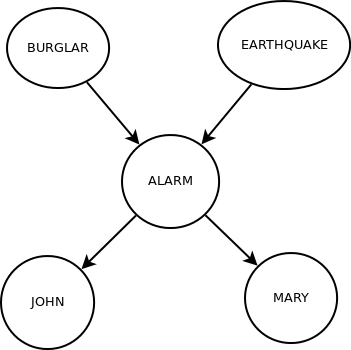
\includegraphics[width=0.4\textwidth]{img/bayes_network.png}
    \caption{An example of a Bayesian network.}
    \label{fig:bayesnet}
  \end{center}
\end{wrapfigure}

\begin{table}[h]%[!htb]
    \begin{minipage}{.25\linewidth}
      %\caption{A burglar entered the house.}
      \centering
        \begin{tabular}{cc}
          \toprule
          $B$ & $P(B)$ \\
          \midrule
          $+b$  & 0.001 \\
          $\neg b$  & 0.999\\
          \bottomrule
          \toprule
          $E$ & $P(E)$ \\
          \midrule
          $+e$  & 0.002 \\
          $\neg e$  & 0.998\\
          \bottomrule
        \end{tabular}
    \end{minipage}%
    \begin{minipage}{.4\linewidth}
      \centering
        %\caption{An earthquake occurred.}
        \begin{tabular}{cccc}
          \toprule
          $B$ & $E$ & $A$ & $P(A|B,E)$\\
          \midrule
          $+b$     & $+e$     & $+a$     & $0.95$ \\
          $+b$     & $+e$     & $\neg a$ & $0.05$ \\
          $+b$     & $\neg e$ & $+a$     & $0.94$ \\
          $+b$     & $\neg e$ & $\neg a$ & $0.96$ \\
          $\neg b$ & $+e$     & $+a$     & $0.29$ \\
          $\neg b$ & $+e$     & $\neg a$ & $0.71$ \\
          $\neg b$ & $\neg e$ & $+a$     & $0.001$ \\
          $\neg b$ & $\neg e$ & $\neg a$ & $0.999$ \\
          \bottomrule
        \end{tabular}
    \end{minipage}
    \begin{minipage}{.35\linewidth}
      %\caption{A burglar entered the house.}
      \centering
        \begin{tabular}{ccc}
          \toprule
          $A$ & $J$ & $P(J|A)$ \\
          \midrule
          $+a$     & $+j$     & $0.9$ \\
          $+a$     & $\neg j$ & $0.1$ \\
          $\neg a$ & $+j$     & $0.05$ \\
          $\neg a$ & $\neg j$ & $0.95$ \\
          \bottomrule
          \toprule
          $A$ & $M$ & $P(M|A)$ \\
          \midrule
          $+a$     & $+m$     & $0.7$ \\
          $+a$     & $\neg m$ & $0.3$ \\
          $\neg a$ & $+m$     & $0.01$ \\
          $\neg a$ & $\neg m$ & $0.99$ \\
          \bottomrule
        \end{tabular}
    \end{minipage}%
    \caption{Probabilities of the Bayesian network in figure \ref{fig:bayesnet}.}
    \label{tab:probsbn}
\end{table}

$P(B)$ and $P(E)$ are, respectively, the probability of a burglar having entered the house, and the probability of having detected an earthquake; $P(A|B,E)$ is the probability that the alarm rings, given we know the status of $B$ and $E$; $P(J|A)$ and $P(M|A)$ are the probabilities that we receive a call from John and Mary, given the status of the alarm. The only ``stand-alone'' probabilities that we can define are the ones of the \textit{evidence} variables (we do know them), namely the burglar and the earthquake. All the other events can only have a probability conditioned to the occurrence of its direct ancestors. To know the probability of one of these events alone, we have to compute the total probability of the event.
With the numbers given in the example, if Mary hasn't called, then the alarm was off w.p. $0.99$. Knowing this, the probability that there has been a burglary is roughly $1.12 \times 10^{-6}$.

We can also read the diagram backward, from bottom to top: for example, $A$ depends on both $J$ and $M$: if the alarm occurs, then it is likey that John or Mary have called.

\subsubsection{Conditional independence}
Given three events $A$, $B$ and $C$, we say that $A$ and $B$ are \textit{conditionally independent} if $P(A \cap B | C) = P(A|C)P(B|C)$, or, equivalently, $P(A | B \cap C) = P(A|B)$. In a bayesian network, two variables (events) are independent if they are not linked by just unknown variables. For example, if we do not know anything about the alarm, then burglary and earthquake are independent, since we cannot infer anything about them.

If the alarm rings, and we know that an earthquake has occurred, then it becomes less likely that a burglar has entered the house, since we already have a cause that can have triggered the alarm. This is the \textit{explaining away} effect.

When an event has multiple causes, then we say that seeing one cause of the possible ones may ``explain away'' all the other causes, because it becomes less likely for them to happen.

\subsection{The \textit{naive} approach}
Bayesian networks require a huge number of variables: because of the chain rule of probabilities, if a node has $k$ incoming arcs, then we need $2^k$ variables. Furthermore, it may difficult to compute the joint probability of variables.

The \textit{naive} approach works under the assumption of independence among variables. It is called ``naive'' since this assumption is very string but not always realistic. Consider now the case of a spam mail: if we read the words ``buy replica watches'' (which already is a set of words) we expect to read some watch brands too. Anyway, while considering all the subset of words requires exponential time, the assumption of independence allows us to consider each word alone, pulling it out of context, and therefore it allows the computation to drop from exponential to linear time. Moreover, the calculation of the probabilities is now reduced to a product of the single probabilities of the variables. Maybe surprisingly, this approach works quite well in practice, being both fast and accurate, despite its ``naivety''.

\subsection{Naive Bayes for spam classification}
We describe now how to apply the theory above to a real problem, in this case the classification of a mail as a spam mail or a valid mail.

We define a mail as \textit{spam} if it contains undesidered or illegal content. A valid mail is conversely defined as \textit{ham}.

The naive approach that tells us to consider each words alone, allows to represent the document as a \textit{bag of words}, which is a dictionary containing the words encountered in the mails, each one associated with its frequency (see figure \ref{fig:nbs}). We read the diagram this way: if we have a mail, what is the probability of reading the word \verb!word1!, knowing the mail is spam? And \verb!word2!? And so on.

\begin{figure}[h]
  \begin{center}
    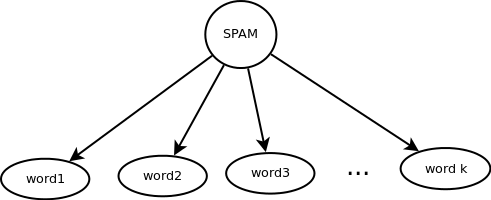
\includegraphics[width=0.6\textwidth]{img/bayes_network_spam.png}
    \caption{An image of a Naive Bayes network for spam classification.}
    \label{fig:nbs}
  \end{center}
\end{figure}

In addiction to the words, often we can easily distinguish a spam email from a valid one by looking at it and recognizing some of these characteristics: bad grammar, bad syntax, undue use of images, lots of links, and many others. Detecting these features may be useful to correctly classify an email.

\subsubsection{Algorithm}
\paragraph{Data structures}
To represent the \textit{bag of words}, we need a dictionary of \verb!(word, stats)!. We need also to store the statistics for the various features detected, in an analogous data structure containing \verb!(feature, stats)!. In both cases, the statistics have to distinguish between frequency in spam mails and frequency in ham mails. This is enough to contain all the informations we need to know about the training set.

The statistics of the mails in the validation set and in the test set will be stored in similar data structures, but their stats will contain only the number of times the words and the featured have been observed, since the network does not know the status of the mail when these operations are performed.

\paragraph{Training}
To train the system, we have to feed the network with the training set. The network will read the mails, extract the actual content and adjust the count of both words and features.

\paragraph{Validation}
The next step is to measure how good the results of the training are. To accomplish this, we provide the network other mails of which we already know the status, to later check the results. The network will read each mail, extract the stats and compare them to the overall statistics generated during the training step. The result of the classification will be the class that maximizes the probability for the mail to belong to that class.

\paragraph{Testing}
Now we compute the final accuracy of the bayesian network, in the same way as the validation, on a larger set of mails.

For both validation and testing, the bayesian network can track its previous work and update the probabilities, so to keep its tables up-to-date and to reflect the actual nature of the dataset.

\subsubsection{Computing the probability}
\label{computeprob}
From the previous sections, we know that for each word $$P_{spam|word} = \frac{P_{word|spam}P_{spam}}{P_{word}}, \quad P_{ham|word} = \frac{P_{word|ham}P_{ham}}{P_{word}}.$$ Since $P_{word}$ is just a normalizer and is the same for both the terms, it can be omitted. Then, when we analyze the training set, we read the words knowing the status of the mail they belong to, and thus at the end of the training step we can say that $$P_{word|spam} = \frac{\mbox{\# occurrences of word in spam mails}}{\mbox{\# total occurrences of word}}, \quad P_{word|ham} = \frac{\mbox{\# occurrences of word in ham mails}}{\mbox{\# total occurrences of word}}.$$

We need to compute these probabilities for each word we encounter when reading a mail. Finally we compute the total probability for the mail of being spam and ham, which, for the naive assumption of independence, will be respectively $$P_{spam} = \prod_{words \in mail} P_{spam|word} \quad\mbox{and}\quad P_{ham} = \prod_{words \in mail} P_{ham|word}.$$ The outcome of the classification will be the class that maximizes these two probabilities.

\subsubsection{Updating the knowledge}
When the Bayesian network classifies a mail, it uses the result to update its knowledge. This can be done just updating the counter of the statistics of the dictionary associated with the network.
